\documentclass[aspectratio=169]{beamer}

% =================================================
% THEME & SETUP
% =================================================
\usetheme[numbering=fraction,progressbar=frametitle]{metropolis}
\setbeamertemplate{navigation symbols}{}

% =================================================
% PACKAGES
% =================================================
\usepackage{amsmath}
\usepackage{amssymb}
\usepackage{booktabs}
\usepackage{graphicx}
\usepackage{tikz}
\usepackage{xcolor}
\usepackage{colortbl}
\usepackage{multicol}
\usetikzlibrary{positioning, arrows.meta, calc, shapes.geometric, fit, backgrounds}

% =================================================
% COLOR PALETTE — deep navy academic
% =================================================
\definecolor{navy}{RGB}{20,40,75}
\definecolor{accent}{RGB}{42,100,180}
\definecolor{accentlight}{RGB}{180,210,245}
\definecolor{darktext}{RGB}{40,40,50}
\definecolor{midtext}{RGB}{90,95,110}
\definecolor{softbg}{RGB}{245,247,250}
\definecolor{cardbg}{RGB}{235,240,248}
\definecolor{wingreen}{RGB}{34,170,90}
\definecolor{lossred}{RGB}{220,60,60}
\definecolor{warnorange}{RGB}{230,150,30}

\setbeamercolor{normal text}{fg=darktext, bg=white}
\setbeamercolor{frametitle}{fg=white, bg=navy}
\setbeamercolor{title}{fg=navy}
\setbeamercolor{progress bar}{fg=accent}
\setbeamercolor{alerted text}{fg=accent}
\setbeamercolor{block title}{fg=white, bg=accent}
\setbeamercolor{block body}{bg=cardbg}

% =================================================
% TYPOGRAPHY
% =================================================
\setbeamerfont{title}{series=\bfseries, size=\LARGE}
\setbeamerfont{frametitle}{series=\bfseries, size=\large}
\setbeamerfont{subtitle}{size=\normalsize}

% =================================================
% META
% =================================================
\title{TD3 for Competitive Air Hockey}
\subtitle{RL Course WS 2025/26 --- Final Project}
\author{Julian Jurcevic \quad $\cdot$ \quad Team: alphabet-td3}
\date{February 2026}

% =================================================
\begin{document}

% -------------------------------------------------
% TITLE SLIDE
% -------------------------------------------------
\begin{frame}[plain]
  \maketitle
\end{frame}

% =================================================
% CONTENT SLIDES
% =================================================

\begin{frame}{Air Hockey Environment}

\begin{columns}[T]

\column{0.50\textwidth}
\textbf{Environment}
\begin{itemize}\setlength\itemsep{3pt}
  \item 2-player Air Hockey (Gymnasium + Box2D)
  \item 4 continuous actions: $x$, $y$, rotation, shoot
  \item 18-dim state: positions, velocities, angles
  \item Reward: $\pm 10$ + shaped proximity reward
\end{itemize}

\column{0.46\textwidth}
\textbf{Key Challenges}
\begin{itemize}\setlength\itemsep{3pt}
  \item \textcolor{lossred}{Non-stationarity}: opponent improves
  \item Fast dynamics + sparse rewards
  \item Overfitting to single opponent
  \item Must combine attack \& defense
\end{itemize}

\end{columns}

\end{frame}

% =================================================
% =================================================

\begin{frame}{TD3 --- Three Key Ideas}

\begin{columns}[T]

\column{0.48\textwidth}

\textbf{1. Clipped Double Q-Learning}
\vspace{0.1cm}

Two critics; target uses the \emph{minimum}:
\[
y = r + \gamma(1{-}d)\;\min_{i=1,2} Q_{\phi_i'}(s', \tilde a')
\]

\vspace{0.2cm}

\textbf{2. Target Policy Smoothing}
\vspace{0.1cm}
\[
\tilde a' = \text{clip}\!\bigl(\pi_{\theta'}(s') + \epsilon,\; {-c},\; c\bigr)
\]

\column{0.48\textwidth}

\textbf{3. Delayed Actor Updates}
\vspace{0.1cm}

\begin{itemize}\setlength\itemsep{2pt}
  \item Critic: every step; Actor: every 2nd
  \item Polyak averaging: $\phi' \leftarrow \tau\,\phi + (1{-}\tau)\,\phi'$
\end{itemize}

\vspace{0.2cm}

\textbf{Architecture}
\vspace{0.1cm}

\begin{itemize}\setlength\itemsep{2pt}
  \item Actor \& twin critics: 2$\times$256 (tanh)
  \item Actor: $a \in [-1,1]^4$
  \item Critics: concatenated $(s, a)$ input
\end{itemize}

\end{columns}

\end{frame}

% =================================================
% =================================================

\begin{frame}{Exploration Noise \& Replay}

\begin{columns}[T]

\column{0.50\textwidth}

\textbf{Noise Annealing}
\vspace{0.15cm}

\[
\sigma_t = \max\!\left(\sigma_0\!\left(1 - \tfrac{t}{T}\right),\; \sigma_{\min}\right)
\]

\begin{itemize}\setlength\itemsep{2pt}
  \item Broad exploration early, exploitation later
  \item Compared: Gaussian, OU, Pink, Uniform
  \item \textbf{Best: OU noise} (temporal correlation)
\end{itemize}

\column{0.46\textwidth}

\textbf{Replay \& Hyperparameters}
\vspace{0.15cm}

\begin{itemize}\setlength\itemsep{2pt}
  \item Uniform replay (300k buffer)
  \item PER tested but \textcolor{lossred}{hurt performance}
\end{itemize}

\vspace{0.2cm}

\footnotesize
\begin{tabular}{ll}
\toprule
$\gamma$ & 0.99 \\
LR (actor/critic) & $2 \times 10^{-4}$ \\
$\tau$ & 0.005 \\
Batch size & 256 \\
Target noise / clip & 0.2 / 0.3 \\
\bottomrule
\end{tabular}

\end{columns}

\end{frame}

% =================================================
% =================================================

\begin{frame}{Three-Stage Curriculum with Self-Play}

\begin{center}
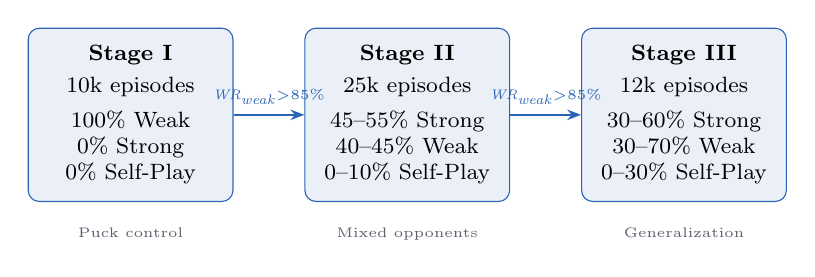
\begin{tikzpicture}[
  stage/.style={
    rectangle, rounded corners=4pt, draw=accent, fill=cardbg,
    minimum width=2.6cm, minimum height=2.2cm, align=center,
    font=\footnotesize
  },
  arr/.style={-{Stealth[length=5pt]}, thick, accent}
]

\node[stage] (s1) {
  \textbf{Stage I}\\[2pt]
  10k episodes\\[3pt]
  100\% Weak\\
  0\% Strong\\
  0\% Self-Play
};

\node[stage, right=0.9cm of s1] (s2) {
  \textbf{Stage II}\\[2pt]
  25k episodes\\[3pt]
  45--55\% Strong\\
  40--45\% Weak\\
  0--10\% Self-Play
};

\node[stage, right=0.9cm of s2] (s3) {
  \textbf{Stage III}\\[2pt]
  12k episodes\\[3pt]
  30--60\% Strong\\
  30--70\% Weak\\
  0--30\% Self-Play
};

\draw[arr] (s1) -- (s2) node[midway, above, font=\tiny\itshape] {WR$_{\text{weak}}{>}85\%$};
\draw[arr] (s2) -- (s3) node[midway, above, font=\tiny\itshape] {WR$_{\text{weak}}{>}85\%$};

\node[below=0.2cm of s1, font=\tiny, midtext] {Puck control};
\node[below=0.2cm of s2, font=\tiny, midtext] {Mixed opponents};
\node[below=0.2cm of s3, font=\tiny, midtext] {Generalization};

\end{tikzpicture}
\end{center}

\vspace{0.15cm}

\textbf{Self-Play Pool:}\;
Snapshots every $k{=}150$ eps $\;\cdot\;$ Pool $N_{\text{pool}}{=}25$
$\;\cdot\;$ Difficulty-weighted sampling ($\times 1.2$ loss, $\times 0.95$ win)

\end{frame}

% =================================================
% =================================================

\begin{frame}{Ablation: Noise Comparison (3 seeds, Stage II)}

\begin{center}
\small
\begin{tabular}{l c c c c}
\toprule
\textbf{Noise Type} & \textbf{WR Weak (\%)} & \textbf{WR Strong (\%)} & \textbf{Ret.\ Weak} & \textbf{Ret.\ Strong} \\
\midrule
Gaussian & 92.5 $\pm$ 4.5 & 81.0 $\pm$ 0.5 & 8.22 $\pm$ 0.80 & 5.69 $\pm$ 0.10 \\
\rowcolor{accentlight}
\textbf{Ornstein--Uhlenbeck} & \textbf{94.7 $\pm$ 0.6} & \textbf{89.0 $\pm$ 2.7} & \textbf{8.56 $\pm$ 0.13} & \textbf{7.06 $\pm$ 0.46} \\
Pink & 92.6 $\pm$ 4.3 & 86.1 $\pm$ 2.8 & 8.17 $\pm$ 0.57 & 6.40 $\pm$ 0.34 \\
Uniform & 91.2 $\pm$ 2.8 & 80.2 $\pm$ 8.4 & 8.10 $\pm$ 0.55 & 5.51 $\pm$ 1.51 \\
\bottomrule
\end{tabular}
\end{center}

\vspace{0.2cm}

\begin{itemize}
  \item OU best: \textbf{+8\%} vs.\ Gaussian against strong (temporal correlation $\rightarrow$ smoother trajectories)
  \item Pink noise second-best (also correlated) $\;\cdot\;$ Uniform: highest variance
\end{itemize}

\end{frame}

% -------------------------------------------------

\begin{frame}{Ablation: Self-Play \& Prioritized Replay (3 seeds)}

\begin{center}
\small
\begin{tabular}{l c c c c}
\toprule
\textbf{Variant} & \textbf{WR Weak (\%)} & \textbf{WR Strong (\%)} & \textbf{Ret.\ Weak} & \textbf{Ret.\ Strong} \\
\midrule
\rowcolor{accentlight}
\textbf{No PER, No SP} & \textbf{93.1 $\pm$ 3.8} & \textbf{78.3 $\pm$ 3.1} & \textbf{8.33 $\pm$ 0.66} & \textbf{5.00 $\pm$ 0.70} \\
No PER, Self-Play & 90.7 $\pm$ 5.9 & 72.6 $\pm$ 7.6 & 7.62 $\pm$ 1.26 & 4.06 $\pm$ 1.56 \\
PER, No SP & 75.8 $\pm$ 9.2 & 66.1 $\pm$ 4.7 & 4.22 $\pm$ 2.00 & 1.99 $\pm$ 1.04 \\
PER, Self-Play & 78.3 $\pm$ 2.2 & 65.3 $\pm$ 5.1 & 4.71 $\pm$ 0.54 & 1.78 $\pm$ 1.01 \\
\bottomrule
\end{tabular}
\end{center}

\vspace{0.15cm}

\begin{columns}[T]
\column{0.48\textwidth}
\textbf{PER} \textcolor{lossred}{hurts performance}
\begin{itemize}
  \item Non-stationary opponents amplify priority variance
  \item $\approx$15--20\% WR drop $\;\Rightarrow\;$ \textbf{not used}
\end{itemize}

\column{0.48\textwidth}
\textbf{Self-Play} --- trade-off
\begin{itemize}
  \item Lower benchmark scores but \textbf{retained} for tournament robustness
  \item Pool diversity decreases as policies converge
\end{itemize}
\end{columns}

\end{frame}

% -------------------------------------------------

\begin{frame}{Curriculum Training Progression}

\textit{Training curves for a representative single-seed run (see report Figure~1).}

\vspace{0.3cm}

\begin{center}
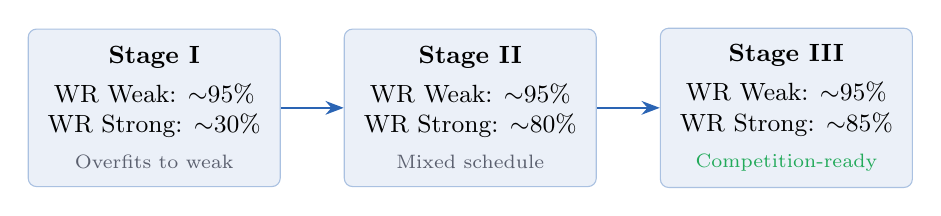
\begin{tikzpicture}[
  card/.style={
    rectangle, rounded corners=3pt, draw=accent!40, fill=cardbg,
    minimum width=3.2cm, minimum height=2.0cm, align=center, font=\small,
    inner sep=6pt
  }
]

\node[card] (c1) {
  \textbf{Stage I}\\[3pt]
  WR Weak: $\sim$95\%\\
  WR Strong: $\sim$30\%\\[2pt]
  {\scriptsize\textcolor{midtext}{Overfits to weak}}
};

\node[card, right=0.8cm of c1] (c2) {
  \textbf{Stage II}\\[3pt]
  WR Weak: $\sim$95\%\\
  WR Strong: $\sim$80\%\\[2pt]
  {\scriptsize\textcolor{midtext}{Mixed schedule}}
};

\node[card, right=0.8cm of c2] (c3) {
  \textbf{Stage III}\\[3pt]
  WR Weak: $\sim$95\%\\
  WR Strong: $\sim$85\%\\[2pt]
  {\scriptsize\textcolor{wingreen}{Competition-ready}}
};

\draw[-{Stealth}, thick, accent] (c1) -- (c2);
\draw[-{Stealth}, thick, accent] (c2) -- (c3);

\end{tikzpicture}
\end{center}

\vspace{0.3cm}

\begin{itemize}
  \item Without curriculum: strong win rate stays at $\sim$30\% (pure weak training)
  \item Staged scheduling resolves this while retaining high weak win rates
  \item Model selection via $\min(\text{WR}_{\text{weak}}, \text{WR}_{\text{strong}})$ enforces robustness
\end{itemize}

\end{frame}

% =================================================
% =================================================

\begin{frame}{Conclusion \& Takeaways}

\begin{columns}[T]

\column{0.55\textwidth}

\textbf{What worked}
\begin{itemize}\setlength\itemsep{4pt}
  \item \textcolor{wingreen}{\textbf{Curriculum}}: most impactful; prevents overfitting to single opponent
  \item \textcolor{wingreen}{\textbf{OU noise}}: +8\% WR (strong) via temporal correlation
  \item \textcolor{wingreen}{\textbf{Self-play}}: retained for tournament generalization
\end{itemize}

\vspace{0.2cm}

\textbf{What didn't work}
\begin{itemize}
  \item \textcolor{lossred}{\textbf{PER}}: $\sim$15\% drop under non-stationarity
\end{itemize}

\column{0.42\textwidth}

\textbf{Final Agent Config}
\vspace{0.15cm}

\footnotesize
\begin{tabular}{ll}
\toprule
Algorithm & TD3 \\
Noise & OU (annealed) \\
Replay & Uniform (300k) \\
Curriculum & 3 stages \\
Self-Play & Pool of 25 \\
\midrule
WR Weak & $\sim$95\% \\
WR Strong & $\sim$85\% \\
\bottomrule
\end{tabular}

\normalsize
\vspace{0.3cm}

\textbf{Limitations}
\begin{itemize}\setlength\itemsep{2pt}
  \footnotesize
  \item Single-seed training curves
  \item Manual curriculum tuning
  \item Self-play pool convergence
\end{itemize}

\end{columns}

\end{frame}

% -------------------------------------------------

\begin{frame}[standout]
  Thank you! \\ \vspace{0.3cm}
  {\normalsize Questions?}
\end{frame}

\end{document}